\chapter{An Overview of the Genome Properties Database, InterPro and InterProScan5} \label{genome-properties} 

The architecture and implementation of Micromeda's components, such as Pygenprop and Micromeda-Client, are tied closely to the structure of the Genome Properties database. Thus, it is pertinent to discuss the database's structure before moving onto other chapters. As mentioned in Section \ref{micromeda-overview}, Micromeda uses Pygenprop to predict the biochemical pathways possessed by an organism. These predictions are made by providing Pygenprop with a copy of the Genome Properties database and the output of running InterProScan5 on the organism's predicted proteins. In addition to discussing the structure of the Genome Properties database, this chapter will also discuss how these pathway predictions are carried out. Specifically, how InterProScan5 performs domain annotation on an organism's proteins and how the Genome Properties database uses these annotations to identify the existence of biochemical pathway steps.

\section{Protein Domains and Their Use as Markers of Enzyme Function}

A protein domain is a conserved part of a protein's sequence that carries out a specific function and is evolutionarily conserved \cite{ren2008conservation}. These domains often generate discrete three-dimensional structures during folding of their host protein \cite{ren2008conservation} and are associated with distinct sequence motifs, which are patterns in the protein's amino acid sequence \cite{ren2008conservation}. An enzyme's function is highly correlated with its domain content \cite{han2007folding}. For example, all enzymes have an active site (\href{en.wikipedia.org/wiki/Active\_site}{en.wikipedia.org/wiki/Active\_site}), a pocket area on its three-dimensional surface that directly interacts with substrates (see Section \ref{enzymes-and-pathways}) and is the site where catalysis takes place \cite{bugg2012introduction}. This active site area has a unique sequence motif that is often uniquely identifiable to specific enzymes or enzyme families \cite{ren2008conservation}. Often proteins consist of a series of domains that are chained together \cite{han2007folding}. For example, a protein that embeds itself within a cell membrane will have domains associated with this trait \footnote{Proteins that have a specific pattern of hydrophobic amino acids on their folded surface tend to embed themselves within cell membranes. Bioinformatics software can easily recognize the motifs associated with this trait  \cite{chen2003secreted,hennerdal2011rapid,von2006membrane}.}. Similar to how different enzymes can be swapped in and out of biochemicals pathways (see Section \ref{enzymes-and-pathways}), domains can also be gained and lost from their host proteins over time and according to evolutionary forces \cite{pasek2006gene}. For example, enzymes that are evolutionarily related may locate differently in the cell due to the presence or absence of the above membrane-associated domains \cite{wang1991existence,hiki1991cytosolic,balasubramanian1992cytosolic}. It is quite common to have some members of an enzyme family cytosolic (i.e., free-floating within the cell) versus others membrane-bound depending on the presence or absence of this domain \cite{wang1991existence,hiki1991cytosolic,balasubramanian1992cytosolic}. Thus, an enzyme's domain content can be used as a marker of both its function and cellular localization.

The Genome Properties database maps between combinations of protein domains and enzymes that carry out pathway steps. \cite{richardson2018genome}. If all the required domains for a pathway step are present in an organism's proteins, then it is considered present. The domains used as markers by the Genome Properties database are those catalogued within the InterPro consortium of protein databases \cite{apweiler2000interpro,richardson2018genome}.

\section{The InterPro Consortium of Protein Databases}

As researchers have accumulated data about enzymes and other types of proteins, protein databases have been developed to catalogue this information. Because many organisms share the same elements of metabolism and the enzymes that carry out these elements are highly similar and often evolutionarily related, it is useful to categorize proteins into groups that carry out a single function or share a specific domain. Protein databases record the function of these groups of proteins and their domains and also store copies of their sequences. In the past, many of these databases were maintained, operated, and funded independently. However, in the past two decades, many of the operators of these protein databases have banded together to form the InterPro consortium \cite{apweiler2000interpro,hunter2008interpro,Hunter2009}, which is headed by the European Bioinformatics Institute (EBI) \cite{cook2015european,finn2016interpro}. As of 2019, the InterPro consortium of protein databases manages fourteen child databases \cite{finn2016interpro,Hunter2009}. Examples of such databases include PFAM \cite{bateman2004pfam}, TIGRFAM \cite{Haft2013}, PANTHER \cite{mi2005panther}, the Conserved Domain Database (CDD) \cite{marchler2014cdd}, HAMAP \cite{lima2008hamap}, PRINTS \cite{attwood2000prints} and many others. In addition to the member databases, the consortium also provides the InterPro database \cite{hunter2008interpro,finn2016interpro}, which is a meta-database that allows for mapping between identical records for the same protein or domain groups across member databases. Each protein or domain catalogued is given a global InterPro identifier (e.g. IPRXXXX) that is mapped to multiple identifiers for the same protein or domain within member databases (e.g. PFXXXX or TFXXXX) \cite{hunter2008interpro,finn2016interpro}. For the most part, each InterPro protein or domain is only catalogued by a subset of member databases within the consortium, not all.

An import feature of protein databases is the ability to take the sequence of a novel protein (i.e., a protein that is not currently in the database) and predict the placement and function of its domains. This process is called domain annotation. Such databases perform this operation by executing sequence similarity searches between the novel protein and domain sequences stored within the database. There are slight differences in a domain's sequence across proteins and organisms and most databases try to capture this sequence diversity. Thus, protein databases catalogue the sequences of multiple representatives of a domain from different proteins and taxonomic groups. When the database is used to domain annotate a novel protein, the search algorithms used to compare the novel protein to a model (i.e., a profile) that represents the sequence diversity (i.e., not all domains in a family have the same sequence) of each domain in the database. If the novel protein possesses a region of high similarity to a model, then it is likely that the novel protein possesses the domain that the model represents. Examples of such modelling approaches include the creation and use of Position-Specific Scoring matrices (PSSMs) \cite{stormo1982use} and hidden Markov models (HMMs) \cite{de2007hidden} that represent a domain's sequence.

\begin{figure}[!ht]
  \centering
	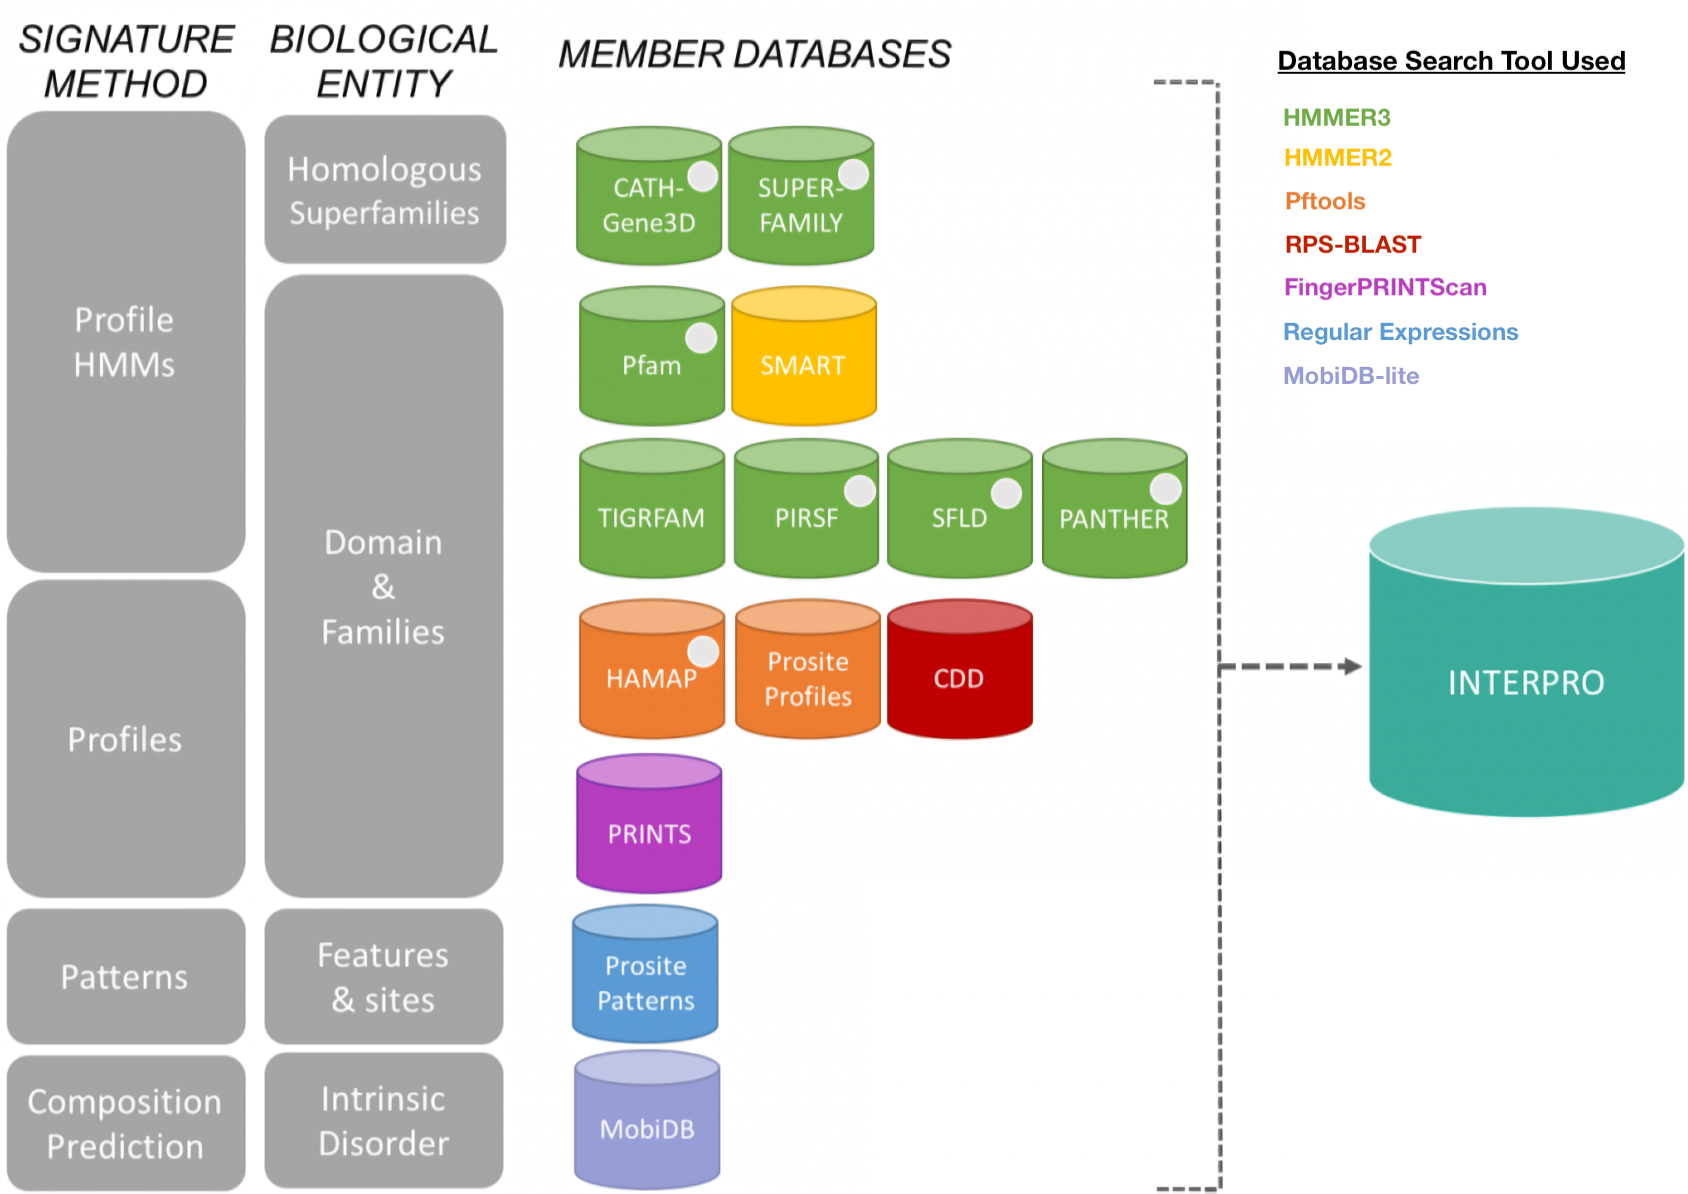
\includegraphics[width=0.90\textwidth]{media/InterPro.png}
	 \caption{The InterPro consortium of protein databases uses a variety of methods to classify novel protein sequences.}
	 \label{fig:interpro-databases}
\end{figure}

Because the member databases of the InterPro consortium were developed independently, the methods they use for sequence search also vary (Fig. \ref{fig:interpro-databases}). The majority of them use HMMER (Fig. \ref{fig:interpro-databases}) \cite{eddy2011accelerated}, which is software that can be used to build an HMM model of a domain's sequence and then use this model to determine if a novel protein is a member of contains the domain. The Conserved Domain Database, another member database, uses pre-calculated PSSMs for different domains and PSIBLAST \cite{altschul1997gapped} to determine if a novel protein possesses the domains that PSSMs represent (Fig. \ref{fig:interpro-databases}).

If a portion of an organism's protein and a model are highly similar in sequence, they form a match. The quality of this match can be quantified by metrics such as the expected value (E-value) score. This E-value score captures how likely it is that the match is a real (i.e., the organism's protein contains the domain) given the chance of finding an equivalent match randomly in one of the organism's other proteins. Another metric for match quality is the length of the region of high sequence similarity, the alignment, shared between the protein and the database domain. Matches with longer alignment lengths are more likely to be real than those with shorter alignment lengths. If it is determined that a match is of high quality, the aligned region of the organism's protein can be assigned the same name and function as the domain in the database. Matches are also known as signatures because they mark the type and placement of a domain. As discussed in Chapter \ref{Pygenprop}, Pygenprop can generate Micromeda files that store such match information.

Each member database has algorithms for filtering out false positive matches, which are those that occur between a domain model and a region of a protein that does not carry out the same function as the domain that the model represents. The member databases perform this filtering by implementing unique cut-off values, such as minimum E-value scores or alignment lengths, that can be used to filter out matches that may be spurious. The cut-off values can be made unique to each model. 


\section{InterProScan}

As member databases were eventually folded into the InterPro consortium, the InterPro consortium created a tool, InterProScan, that allows users to compare a novel protein sequence to all domain models found within InterPro member databases. InterProScan is a software wrapper for and execution engine of the model-based sequence search techniques (e.g. HMMER or PSIBLAST) used by all member databases of the InterPro consortium. It also implements the false positive filtering techniques developed for each member database. Thus, InterProScan can be used as a domain annotator. The latest version of the software, InterProScan5, follows a Master/Worker architecture (see \href{https://en.wikipedia.org/wiki/Master/slave\_(technology)}{https://en.wikipedia.org/wiki/Master/slave\_(technology)}) where a master process schedules jobs for many worker processes. Each of these jobs compares a novel protein to a single database model using the model's matching search tool. Depending on the number of CPU cores of the computer running InterProScan5, tens to hundreds of models can be run against a novel protein simultaneously. Due to its Master/Worker architecture, InterProScan5 can also run jobs run across a computer cluster with one master process on a single machine controlling worker processes on machines across a network. Due to this scalability, InterProScan is capable of domain annotating every protein of a microorganism in only a few hours, depending on the computer it is run on an organism's genome size. InterProScan takes a FASTA file \cite{pearson19905} containing an organism's predicted proteins (as would be created by Prodigal) as input and writes domain annotations and match data to tab-separated value (TSV) files. The match data includes supporting information such as E-value scores for matches and predicted domain start and stop points on the organism's annotated protein.

\section{The Genome Properties Database}

The backbone of Micromeda is the Genome Properties \cite{Haft2013} database. The database goes beyond simple metabolism to include other organism capabilities such as cell motility (e.g. the presence flagella) and even microbial viral immunity mechanisms such a CRISPR/Cas \cite{horvath2010crispr}. Multiple steps support each property, and each of these is supported by multiple pieces of evidence found within an organism's predicted proteins. Precisely, matches to InterPro domains. The initial versions of the Genome Properties database were developed by the J. Craig Venter Institute (JCVI) to support the Comprehensive Microbial Resource (CMR) \cite{Davidsen2010}, an annotation web server that was later shut down in the mid-2010s. Early versions of the Genome Properties databased relied solely on matches to TIGRFAM HMMs \cite{Haft2013, Novere2009}. These matches were used to assess support for an organism possessing specific properties. On the shut down of the CMR, the Genome Properties database was transferred \cite{finn2018} to the InterPro consortium \cite{Hunter2009}. TIGRFAM also became a member database of the consortium around this time. Rather than only using matches to TIGRFAM HMMs, the Genome Properties database was transitioned to use any InterPro domain model (e.g. PFAM or CDD domains) as evidence. One of the core goals of the latest release of Genome Properties was to expand the database beyond prokaryotic properties to include properties that are only possessed by eukaryotes or are shared between prokaryotes and eukaryotes. This shift was one of the core reasons why the database was transitioned to use any InterPro model rather than just TIGRFAM HMMs. TIGRFAM models were tailored to identifying prokaryotic proteins \cite{Haft2013}. However, other member databases contain more general models. The most recent version of the Genome Properties database has also incorporated pathways from MetaCyc \cite{karp2002metacyc}, under special permission from this database's creators.

\subsection{The Structure of the Genome Properties Database}

Multiple steps support each property within the Genome Properties database, and multiple lines of evidence support each of these. If a specified number of required steps are found within the domain annotations of an organism's proteins, then the organism is understood to posses a specific genome property. Some genome properties are required as lines of evidence by others, and thus the database forms a rooted directed acyclic graph (DAG) of connected properties. There are five types of genome properties: pathways, metapathways, systems, guilds and categories (see Table \ref{tab:property-types}). 

\begin{longtable}[c]{|p{2.5cm}|p{13cm}|}
\caption{There are currently five types of genome properties. This table is from the Genome Properties database documentation (\href{genome-properties.readthedocs.io/en/latest/flatfile.html}{genome-properties.readthedocs.io/en/latest/flatfile.html}).}
\label{tab:property-types}\\
\hline
\textbf{Property Type} & \textbf{Description} \\ \hline
\endfirsthead
%
\multicolumn{2}{c}%
{{\bfseries Table \thetable\ continued from previous page}} \\
\hline
\textbf{Property Type} & \textbf{Description} \\ \hline
\endhead
%
PATHWAY & These represent groups of proteins that perform biochemical steps in order within a recognised enzymatic pathway. \\ \hline
METAPATH & These represent a specific type of PATHWAY where one or more of the steps within the pathway are described by another [g]enome [p]roperty. For the purposes of calculation, METAPATHs are dependent on their respective [genome property] steps. \\ \hline
SYSTEM & These represent groups of proteins that work together to fulfil a role, but do not necessarily represent a traditional enzymatic pathway (for example, transport systems). \\ \hline
COMPLEX & These represent stable macromolecular complexes. \\ \hline
GUILD & These represent groups of proteins sharing overall function, but which do not represent a system. \\ \hline
CATEGORY & These are organisational properties that allow the full set of genome properties to be arranged into a hierarchy. \\ \hline
\end{longtable}

Pygenprop contains code for generating object-oriented classes that represent individual properties, steps and pieces of evidence of the Genome Properties database. It also provides a class for representing the entire database. Objects of this class, built from a provided copy of the Genome Properties database, can be used to quickly lookup information on individual properties and discover the pieces of evidence used to support them. The classes are further detailed in Section \ref{genomeprop-oop}.

\subsection{Assignment of Genome Properties to an Organism}

To assign properties to an organism, InterProScan is first used to domain annotate all of its predicted proteins (e.g. those produced by Prodigal), and these annotations are then combined with information from the Genome Properties database to assess which properties are supported. Each property in the database is assigned YES, PARTIAL and NO support. With Micromeda, Pygenprop is used to carry out these assessments. Genome Properties database is provided to Pygenprop in the form of a release file, whose contents are detailed in the section below. Section \ref{AssignmentCachingAlgorithm} details the exact algorithms used for generating assignments.  

\subsection{Overview of the Genome Properties Flat File Database and Associated File Formats} \label{Genome-Properties-Files} 

The Genome Properties database (as of version 2.0) consists of a series of flat files that are hosted inside a Github repository (see \href{github.com/ebi-pf-team/genome-properties}{github.com/ebi-pf-team/genome-properties}). Information about individual properties is stored in the repository's \textbf{data} folder, and within this folder, each property is assigned a second internal folder containing three files: 
\begin{itemize}
\item A \textbf{DESC} file, that contains information about the property
\item A \textbf{status} file that contains information onto whether the property is public or has been manually curated
\item A \textbf{FASTA} \cite{pearson19905} file containing representative protein sequences that carry out the steps a the property
\end{itemize}
The \textbf{data} folder contains information about both public and non-public genome properties. 

In addition to the per-property folders, there is also a Genome Properties release file located in the \textbf{flatfiles} folder of the repository that also contains Genome Properties information. Specifically, this file, called \textbf{genomeProperties.txt}, is a concatenation of all the \textbf{DESC} files of all public properties. This file is created with each new release of the Genome Properties database on Github. Below is simplified a folder structure for the Genome Properties Github repository.

\begin{verbatim}
├── code/ - # The Genome Properties Perl library.
├── data/ - # Data about both public and private properties
│ ├── GenProp0001/
│ │ ├── DESC - # Detailed property information
│ │ ├── FASTA - # Sequences of proteins that carry out steps
│ │ └── status - # Public and manual curation status
│ └── GenProp0002/
│  ├── DESC
│  ├── FASTA
│  └── status
└── flatfiles/
 └── genomeProperties.txt
\end{verbatim}

The Genome Properties database parser is capable of parsing both single \textbf{DESC} files of individual properties and the concatenated \textbf{genomeProperties.txt} release file. The format of \textbf{DESC} files is very similar to the Stockholm sequence alignment format used by both the Pfam and Rfam databases \cite{bateman2004pfam, griffiths2003rfam}. Like these file types, \textbf{DESC} files consist of a series of key-value pairs. Because these files use different keys than Stockholm, a custom parser had to be developed. It is of note that the Genome Properties database format wraps every eighty characters. Thus, some key types that contain long sentences are repeated for multiple lines and the parser must unwrap these lines to prevent parsing errors. Below is an example \textbf{DESC} file and a summary of key types can be found in Table \ref{table:property-file-keys}.

\begin{verbatim}
AC GenProp0145
DE Histidine degradation to glutamate
TP PATHWAY
AU Haft DH
TH 2
RN [1]
RM 2203753
RT Nucleotide sequence of the gene encoding the repressor for the
RT histidine utilization genes of Pseudomonas putida.
RA Allison SL, Phillips AT;
RL J Bacteriol. 1990;172:5470-5476.
RN [2]
RM 25559274
RT Structure of N-formimino-L-glutamate iminohydrolase from Pseudomonas 
RT aeruginosa.
RA Fedorov AA, Martí-Arbona R, Nemmara VV, Hitchcock D, Fedorov EV, Almo SC, 
RA Raushel FM;
RL Biochemistry. 2015;54(3):890-7.
DC Histidine Catabolism
DR IUBMB; AminoAcid; His3;
DC Histidine Metabolism
DR KEGG; map00340;
DC L-histidine degradation II
DR MetaCyc; PWY-5028;
CC This pathway is involved in histidine utilization system (hut). HutP is
CC the first gene in the hut operon encoding the hutHUIG operator and a
CC positive regulator of the operon, activated allostatically in the
CC presence of L-histidine. HutC represses histidine utilization by binding 
CC the regulatory sites for hutHUIG and hutF [1]. There are multiple
CC variations in the histidine degradation pathway, including two possible 
CC routes for the first step (either via histidine transaminase, or as in 
CC this pathway, via histidine ammonia-lyase/histidase). L-histidine is 
CC first converted to urocanate by hutH (histidine ammonia-lyase), that is 
CC then converted to 4-imidazolone-5-propionate by hutU (urocanate 
CC hydratase), and finally hydrolysed to N-formimino-L-glutamate by hutI 
CC (imidazolonepropionate amidohydrolase). From here there are three 
CC potential paths to glutamate. This property refers to the two-step 
CC process found in some bacteria where N-formimino-L-glutamate is first 
CC converted to N-formyl-l-glutamate by hutF (formimidoylglutamate 
CC deiminase) and then hydrolyzed to L-glutamate by hutG 
CC (N-formyl-l-glutamate deformylase)[2].
** Evidence for steps 4 and 5 is the same.
--
SN 1
ID Histidine ammonia-lyase (hutH)
DN Histidine ammonia-lyase/hutH (EC 4.3.1.3)
RQ 1
EV IPR005921; TIGR01225; sufficient;
TG GO:0006548;
--
SN 2
ID Urocanate hydratase (hutU)
DN Urocanate hydratase/hutU (EC 4.2.1.49)
RQ 1
EV IPR023637; TIGR01228; sufficient;
TG GO:0006548;
--
SN 3
ID Imidazolonepropionase (hutI)
DN Imidazolonepropionase/hutI (EC 3.5.2.7)
RQ 1
EV IPR005920; TIGR01224; sufficient;
TG GO:0006548;
--
SN 4
ID Formimidoylglutamate deiminase/formiminoglutamase/glu-formyltransferase
DN Formimidoylglutamate deiminase/hutF (EC 3.5.3.13)
RQ 1
EV IPR005923; TIGR01227; sufficient;
TG GO:0006548;
EV IPR010252; TIGR02022; sufficient;
TG GO:0006548;
EV IPR004227; TIGR02024; sufficient;
TG GO:0006548;
--
SN 5
ID Formylglutamate deformylase/formiminoglutamase/glu-formyltransferase
DN N-formylglutamate deformylase/hutG (EC 3.5.1.68)
RQ 1
EV IPR005923; TIGR01227; sufficient;
TG GO:0006548;
EV IPR010247; TIGR02017; sufficient;
TG GO:0006548;
EV IPR004227; TIGR02024; sufficient;
TG GO:0006548;
--
SN 6
ID Histidine utilization repressor (hutC)
DN Histidine utilization repressor/hutC
RQ 0
EV IPR010248; TIGR02018; sufficient;
//
\end{verbatim}

\begin{longtable}{|l|l|}
\caption{Genome Properties \textbf{DESC} files use a variety of keys to provide information about a single property. The below table is copied from the Genome Properties database \href{genome-properties.readthedocs.io/en/latest/flatfile.html\#desc-file}{documentation}.}
\label{table:property-file-keys}\\
\hline
\textbf{Key} & \textbf{Information Type} \\ \hline
\endfirsthead
%
\multicolumn{2}{c}%
{{\bfseries Table \thetable\ continued from previous page}} \\
\hline
\textbf{Key} & \textbf{Information Type} \\ \hline
\endhead
%
AC & Accession ID \\ \hline
DE & Description/name of Genome Property \\ \hline
TP & Type \\ \hline
AU & Author \\ \hline
TH & Threshold \\ \hline
RN & Reference number \\ \hline
RM & PMID of reference \\ \hline
RT & Reference title \\ \hline
RA & Reference author \\ \hline
RL & Reference citation \\ \hline
DC & Database title \\ \hline
DR & Database link \\ \hline
PN & Parent accession ID \\ \hline
CC & Property description \\ \hline
** & Private notes \\ \hline
– & Separator \\ \hline
SN & Step number \\ \hline
ID & Step ID \\ \hline
DN & Step display name (includes EC number if available) \\ \hline
RQ & Required step \\ \hline
EV & Evidence (includes whether sufficient) \\ \hline
TG & Gene Ontology (GO) ID \\ \hline
// & End \\ \hline
\end{longtable}

\subsection{Reasoning for the Selection of Genome Properties as Micromeda's Pathway Information Source}

During the development of Micromeda, there were four reasons for selecting the Genome Properties database over other databases. These reasons are laid out below.

First, the majority of alternative pipelines for pathway annotation identify enzymes via sequence similarity search tools such as BLAST \cite{altschul1990basic}, which compare an organism's proteins to a single representative enzyme sequence that that is known to carry out a pathway step. In contrast, the pathway annotations created Micromeda, using the Genome Properties database, are built on top of domain annotations created by HMMER or PSIBLAST, which are model-based approaches. As compared to BLAST-based search methods, these model-based approaches are better at detecting enzymes whose sequences are phylogenetically divergent from those previously known \cite{eddy2011accelerated} \footnote{Model-based approaches provide better detection because they can bias match scores by emphasizing the presence of some areas of a protein's sequence over others \cite{eddy2011accelerated}. For example, the active site motif of an enzyme's sequence, which is highly conserved, is often emphasized over other regions in these models. This biasing would cause a novel protein that retains a highly similar active site to the modelled protein to be given increased match scores as compared to a protein that has a different active site. In contrast, BLAST treats all positions on a protein's sequence as equal, which de-emphasizes these conserved regions. Thus, model-based approaches are better at detecting remotely homologous enzymes whose overall sequence is quite remote, but whose active site and thus function has not changed \cite{eddy2011accelerated}.}. These approaches also provide better true positive detection \cite{eddy2011accelerated}.

Second, because the Genome Properties database is domain-based rather than whole protein sequence-based, Micromeda can detect the presence of enzymes that are split across two genes or have fused with other proteins. In a recent study that focused on confirming genome-predicted amino-acid auxotrophy (i.e., inability to produce essential amino acids) across a variety of bacteria, the authors found that many predicted instances of auxotrophy were misannotations \cite{price2018filling}. Many of these misannotations were the result of either gene fusions or the enzyme being split across multiple genes \cite{price2018filling}. Traditional whole protein sequence-based detection methods using BLAST, as is typical for pathway annotation pipelines based on databases such as KEGG, were shown in the above publication to miss these enzymes \cite{price2018filling}. For example, if previous forms of an enzyme were all found to be encoded by a single gene, such whole sequence methods may filter out versions of the enzyme that are split across genes due to inadequate alignment lengths for matches to individual subunits \cite{price2018filling}. In contrast, Micromeda would determine that the enzymes exist, as InterProScan will pick up all required domains, whether the enzymes are on one gene or multiple.

Third, two of the most prominent pathway databases, KEGG and BioCyc \cite{karp2005expansion}, have been commercialized by companies such as Pathway Solutions and Phoenix Bioinformatics, respectively. KEGG's website is free for academic use in terms of using the data held within for hypothesis testing (see \href{www.kegg.jp/kegg/legal.html}{kegg.jp/kegg/legal.html}). However, bulk download of the entire database, as would be required for any pathway annotation system such as Micromeda, has a licensing fee of \$2000 USD per year (as of 2019 and see \href{bioinformatics.jp/docs/subscription\_fees.pdf}{bioinformatics.jp/docs/subscription\_fees.pdf}). This fee increases to \$5000 per year if a user "provide[s] any outside service using... KEGG data" (as of 2019 and see \href{bioinformatics.jp/docs/subscription\_fees.pdf}{bioinformatics.jp/docs/subscription\_fees.pdf}). Thus, if Micromeda were built around the KEGG database, users creating Micromeda files would be required to pay \$2000 USD per year, and any user hosting Micromeda server, as a public service, would be required to pay \$5000 per year. BioCyc follows a similar paid scheme (\href{metacyc.org/download.shtml}{metacyc.org/download.shtml}). For commercial users, such fees are an order of magnitude higher. In contrast, the Genome Properties database is freely available under an open-source licence and is hosted on Github \cite{richardson2018genome}.

Finally, a common way of assessing the completeness of a pathway database is to perform pathway annotation on a variety of phylogenetically distant organisms to determine how many of these organisms' proteins contribute to pathways found within the database. The ratio of these proteins to those unknown to the database provides a snapshot of the database's completeness. A pathway database that is highly complete should cover the majority of these organisms' proteins. The Genome Properties database has been shown to have comparable coverage, in terms of organism proteins used to support the existence of pathways, to databases such a KEGG and Seed Subsystems \cite{richardson2018genome}. This coverage was consistent across a variety of microbes from distant taxonomic clades \cite{richardson2018genome}. Thus there is no high-level database completeness disadvantage if Micromeda uses the Genome Properties database. 

\section{Summary}

When Micromeda performs pathway annotation, it does so based on the presence of InterPro domains found within organisms' predicted proteomes. These domains are detected using model-based sequence search software that is orchestrated by InterProScan5. The contents of the Genome Properties database is used to map from the presence of domains to the presence of genome property steps. The presence of steps is used to infer YES, PARTIAL or NO support for individual genome properties. The model-based search techniques used by InterProScan allow Micromeda to provide highly accurate and comprehensive results with no licensing fees.